In this chapter we will specify with detail the system requirements and particular features to be implemented. The requirements
will be divided in two major sections.\\
\indent First we will describe what tasks the Back-end of the system should perform in order to provide
all the data and tools for supporting the system Front-end. Then with the end user in mind we will define the tool requirements from
the user point of view. For aggregator that is part of the Front-end no requirements will be specified since this component will only bridge
requests from the Front-end and the Back-end or will eventually fetch data directly from the database.\\

\section{Social Networks Prioritization}
Before diving into the requirements we first will review our \glspl{osn} preferences regarding information extraction and the
interest we have in analyzing this specific networks.\\
\indent First we want to analyze \textbf{Facebook} because it is the more general purpose network, the more popular and the more used
thus allowing us to derive more interesting conclusions since the resultant graphs will be more realistic having a more concrete social structure
representation. Second we want to analyze \textbf{LinkedIn} because it is also widely used and the only one that specifically
focus on professional worldwide networking, generating different kinds of graphs and understand how companies and professionals
are interacting online. Analyzing LinkedIn may also introduce an interesting analysis that is merging information from Facebook and
analyzing friendship networks within professional networks.\\
\indent Having two networks embedded in the system proves that we can analyze social networks in general since we have more
than one and with different purposes, but since the system is designed to simply accommodate new networks simply adding
a new extraction module should the major part of the work to integrate a new \glspl{osn}, this said we could eventually
also implement some extra modules to the remaining \glspl{osn} listed in chapter 3.

%% ---------------------------------------------- Back-end
\section{Back-end}

As seen is Figure \ref{img:architectureprop}, our Back-end is essentially composed by two parts: \textbf{web crawlers/extraction modules}; \textbf{extraction manager} and the \textbf{data miner}. We will write the requirements for each one of the components. We will not prioritize these requirements (as we will do in the \hyperref[sec:frontend]{next section for the Front-end} requirements) because \textbf{all listed requirements are essential for the overall system usefulness}.

\subsection{Web crawlers}

Each web crawler (or extraction module) must fulfill common requirements that are listed below \footnote{These requirements are agnostic to the \glspl{osn} context}:

\begin{enumerate}
    \item Web crawlers should be able to login with a user account (an \textit{entry point});
    \item Web crawlers should be able to navigate through the pages of a given \gls{osn};
    \item Web crawlers must be capable of performing "human" interactions such as click and scroll;
    \item Web crawlers should be able to output a predefined (agreed and formally defined in the next section) data schema, covering eventual
    exceptions due to privacy limitations;
    \item Web crawlers must be able to perform user extraction with second order depth, from the user entry point perspective (this means that we want to extract user's friends and friends of friends information);
    \item Extraction modules should provide a global extraction method where extraction parameters can be passed from the outside reducing or amplifying the scope of extraction as specified from the outside (e.g. under given circumstances we may only need to extract the friends' list or the basic information like name, city and birth date);
    \item Extraction modules must be available to the data miner through a web \gls{api} in order to allow remote and distributed extraction. The web \gls{api} must wrap all the different supported \glspl{osn} being each one accessible through a different path within the same web \gls{api}. The extraction web \gls{api} required specifications are presented next:
    \begin{itemize}
        \item \textbf{GET /api/v1/extraction/\{osn\}} - should return a confirmation message signalizing that \gls{api} is up and ready for receiving requests;
        \item \textbf{GET /api/v1/extraction/\{osn\}/\{user\_id\}} - should perform full extraction of the user with the \textit{user\_id} in the \textit{osn} ;
        \item \textbf{POST /api/v1/extraction/\{osn\}/\{user\_id\}} - should receive a set of options, that parameterize the extraction and reduce the scope of the extraction for a given \textit{user\_id} within some \textit{osn}.
        \item \textbf{POST /api/v1/extraction/\{osn\}/} - same as the previous but instead of performing extraction for a given \textit{user\_id}, performs it to a set of \textit{user\_ids} performing multiple extractions;
        \item In \gls{api} version 1 \textbf{osn} must be one of the following: \textbf{facebook}, \textbf{linkedin};
        \item \textbf{user\_id} is a string that uniquely represents the user within a specific \gls{osn}.
    \end{itemize}
\end{enumerate}

\subsection{Extraction Manager}

Below are the extraction manager requirements \footnote{Again, these requirements are agnostic to the \glspl{osn} context}:

\begin{enumerate}
    \item Orchestration of extraction processes scattered across various hosts: one should be able to define a list of hosts and the number of extraction processes that each host should handle;
    \item Chunk an entry point (that is a set of user identifiers within the \glspl{osn}) in order to delegate different users to different hosts;
    \item Call the extraction endpoints according to the \glspl{osn} from where we need to extract data.
\end{enumerate}

\subsubsection{Extraction pipeline}

\begin{figure}[h!]
\begin{center}
  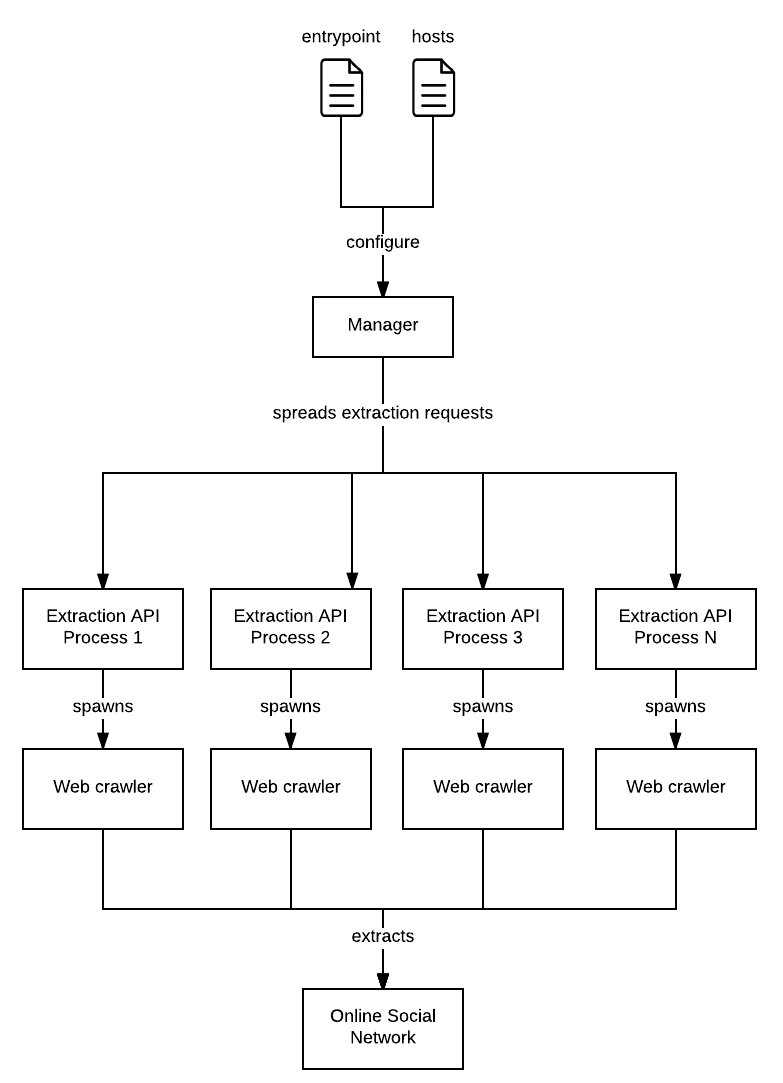
\includegraphics[width=0.7\textwidth]{img/ext-pipeline.png}
\end{center}
\caption{\label{img:extpipeline} Extraction pipeline diagram.}
\end{figure}

Being listed above the requirements for each component we will now draw the specification of what is the expected workflow for data extraction, in Figure \ref{img:extpipeline} we design a pipeline that tries to reflect, with maximum detail, the listed requirements. The diagram does not cover the data mining process that is responsible for normalizing data and store it. This diagram is exclusively focused on how we pretend that data extraction is achieved in order to mitigate the slowness of web crawlers.\\
\indent As we can see from Figure \ref{img:extpipeline} we aim to follow a very straight forward process in order to extract information. First we provide an entry point for a given \glspl{osn} (the user the web crawlers will use to log in into the social platform), and a hosts file that describes the resources available for extractions, this is intended to be simply a list of hosts (ip addresses) that have the extraction web \gls{api} running and awaiting for extraction requests.\\
\indent Next each extraction \gls{api} instance is responsible for handling a session of some web crawler instance and waits for it to return data so the extraction API instance  can give it back to the extraction manager.

\clearpage

\subsection{Data miner}
\label{sec:dataminer}

The data miner simply assures some data treatment before storing it on the database, that said there is a very narrow requirements list for this component:

\begin{enumerate}
\item Receive extraction data and normalize the fields that may need some treatment giving as result a normalized data structure;
\item Store normalized data in the database;
\item Assure that the data schemas (these are presented in the next section) are well defined.
\end{enumerate}

\subsubsection{Data schemas}

Defining data schemas in earlier stages of system specifications will allow us to develop the Front-end and the Back-end simultaneously, we must for that consider that the only source of true when it comes to data structures is a well agreed contract between both parts. The data miner will assure that the next presented schemas are stored in the database. For convenience reasons we will describe the data structures with a JSON like notation.

\subsubsection{Facebook data structure}
\begin{verbatim}
{
    "uid": {string},
    "livesIn": {
        "id": {string},
        "description": {string}
    },
    "life_events": {
        {string}: [{string}]
    },
    "birthDate": {string},
    "likes": {
        {string}: {string}
    },
    "friends": [{string}],
    "relationships": {
        "civil_status": {
            "id": {string},
            "description": {string}
        },
        "family_members": [
            { "id": {string}, "relationship": {string} }
        ]
    },
    "from": {
        "id": {string},
        "description": {string}
    },
    "name": {string},,
    "gender": {string},
    "age": {number},
    "posts": [
        {
            "timestamp": {string},
            "description": {string},
            "author": {string},
            "reactions": {
                "likes": {number},
                "love": {number},
                "laugh": {number},
                "sad": {number},
                "angry": {number},
                "surprise": {number}
            }
        }
    ]
}
\end{verbatim}

\subsubsection{LinkedIn data structure}
\begin{verbatim}
{
    "uid": {string},
    "name": {string},
    "headline": {string},
    "from": {string},
    "summary": {string},
    "experience": [
        {
            "company": {string},
            "position": {string},
            "duration": {
                "count": {number},
                "unit": {string},
                "from": {string},
                "to": {string}"
            }
        }
    ],
    "education": [
        {
            "institution": {string},
            "course": {string},
            "startYear": {number},
            "endYear": {number}
        }
    ],
    "skills": {
        {string}: {number}
    },
    "languages": {
        {string}: {string}
    },
    "projects": [
        {
            "name": {string},
            "date": {string},
            "description": {string}
        }
    ],
    "groups": [
        {string}
    ],
    "following": [
        {string}
    ],
    "connections": [
        {string}
    ]
}
\end{verbatim}

\subsection{Network metrics}
\label{subsec:networkmetrics}

In this section we will list the requirements for the module that is responsible for calculating metrics upon our stored networks. This component must
provide a web \gls{api} in order to access all the algorithms and metrics calculations that the service offers.

\begin{enumerate}
    \item The \gls{api} must be able to calculate strongly and weakly connected components;
    \item The \gls{api} must be able to calculate the clustering coefficient for a given network;
    \item The \gls{api} must be able to calculate the average neighbor degree;
    \item The \gls{api} must be able to calculate centrality measures, these include:
    \begin{enumerate}
        \item Degree centrality;
        \item Closeness centrality;
        \item Betweenness centrality;
        \item Eigenvector centrality;
    \end{enumerate}
    \item The \gls{api} must be able to compute node importance through the page rank algorithm.
\end{enumerate}


%% ---------------------------------------------- Front-end
% This should be one of my major arguments when talking on static rendering and network perception through time!
% https://en.wikiquote.org/wiki/Edsger_W._Dijkstra - Related cool stuff
% Our intellectual powers are rather geared to master static relations and that our powers to visualize processes evolving in time are relatively poorly developed. For that reason we should do (as wise programmers aware of our limitations) our utmost to shorten the conceptual gap between the static program and the dynamic process, to make the correspondence between the program (spread out in text space) and the process (spread out in time) as trivial as possible.
% \textbf{\textit{"You can think of networks as vast fabrics of humanity, and we all occupy particular spots within the network. Nicholas Christakis}} \url{https://www.youtube.com/watch?v=wadBvDPeE4E&t=1133s}"

\section{Front-end}
\label{sec:frontend}

The Front-end is actually where the majority of the requirements work is, since we need to go into detail of how the user will interact with the tool, we must decide how those interactions will be drawn so that the tool can actually be what it was meant to, also bear in mind that these represent the tool requirements, what the user actually will able to see.

\subsection{Requirements Prioritization}
For simplifying the prioritization process we will use the \textbf{MoSCoW} method \citep{clegg1994case} that is a simple method to define what requirements are more important for the system overall functionality, allowing us to focus on the very essential requirements for getting a functional product \footnote{In this section we will tend to use some terms often find in requirements engineering that may seem a bit off topic, still we find that this is the more objective way for describing our prioritization method}.\\
\indent Next we present the MoSCoW method as it is defined in requirements engineering.

\begin{itemize}
    \item \textit{\textbf{M}ust} have requirements are critical requirements that are part of the identity of the product, they must by all means be implemented.
    \item \textit{\textbf{S}hould} have requirements are definitely important, but they are not critic to the product definition, and they are not time critic as well having the possibility of being included in later stages of the implementation. Some times these requirements may have another ways of satisfying the customer.
    \item \textit{\textbf{C}ould} have requirements are indeed the \textit{nice to have} requirements, being often left outside of the first deliver, but seen as very valuable to the future of the product in later stages of the product time line.
    \item \textit{\textbf{W}on't} have requirements that are agreed to not be included in the first deliver of a project, this does not exclude the possibility of including them in later stages of the project. \textit{Won't} requirements may be seen as future work.
\end{itemize}

The requirements will be listed by groups (sections) that aggregate common requirements or features. Each requirement will have a classification according the MoSCoW method.

\subsection{Network configuration and construction}

In this group of requirements we present a set of requirements that represent the operations that allow the users to get their network built.

\begin{enumerate}
    \item \textbf{[MUST]} The user must be able to generate a network for available \glspl{osn};
    \item \textbf{[MUST]} The user must be able to choose the number of nodes for a certain network and which metrics he wants to compute for that network;
    \item \textbf{[MUST]} The user must be able to register available \glspl{osn} accounts in the system;
    \item \textbf{[MUST]} The user must be able to order the build of its network for a given \gls{osn};
    \item \textbf{[MUST]} The system must give feedback on the extraction status;
    \item \textbf{[COULD]} The user must be able to \textit{blacklist} from the network nodes with a minimum or maximum number of connections;
    \item \textbf{[COULD]} The system must clearly warn the user about the impacts that extracting some kind of data (e.g. extracting complete list of user's likes on Facebook) could have on extraction time and consequently on render network time (these could be expressed via label warnings in the user's interface);
    \item \textbf{[COULD]} The user must be able to \textit{blacklist} nodes specific from being extracted and consequently rendered on the user's graph;
    \item \textbf{[WON'T]} After the first extraction all the extracted nodes must be marked as extracted, being the user able to extract the missing properties for some given nodes.
\end{enumerate}
% Extraction granularity
% \begin{enumerate}
%     \item \textbf{Facebook}:
%     \begin{enumerate}
%         \item \textit{Relationships} - If this flag is checked, relationships will be included;
%         \item \textit{Personal} details - If this flag is checked, personal details will be included;
%         \item \textit{Life events} - If this flag is checked, life events will be included;
%         \item \textit{Posts} - If this flag is checked, most recent posts will be included.
%     \end{enumerate}
%     \item \textbf{LinkedIn}:
%     \begin{enumerate}
%         \item \textit{Experience} - If this flag is checked, experience will be included;
%         \item \textit{Education} - If this flag is checked, education will be included;
%         \item \textit{Skills} - If this flag is checked, skills will be included;
%         \item \textit{Languages} - If this flag is checked, languages will be included;
%         \item \textit{Projects} - If this flag is checked, projects will be included;
%         \item \textit{Groups} - If this flag is checked, groups will be included;
%         \item \textit{Connections} - If this flag is checked, connections will be included.
%         \item \textit{following} - If this flag is checked, following will be included.
%     \end{enumerate}
% \end{enumerate}

\subsection{General interactions and display}

These requirements express general behavior of the tool, and some display features.

\begin{enumerate}
    \item \textbf{[MUST]} The system must be able to render a graph using the information provided by the aggregation service;
    \item \textbf{[MUST]} The system should be able to automatically identify communities by painting nodes belonging to the same community by the same color and providing
    information about the community such as \textit{"People that studied at School/University X"} or \textit{"People that live in city Y"};
    \item \textbf{[MUST]} The user must be able to drag and drop the graph to any place on the graph render area;
    \item \textbf{[MUST]} The user must be able to zoom in and zoom out the network so he is able to explore specific parts with more detail;
    \item \textbf{[MUST]} The user must be able to select two nodes at the same time in order to compare them all values should be displayed side by side in order to provide a practical way to compare two individuals at any level;
    \item \textbf{[SHOULD]} The user should be able to choose activate animations despite these have been deactivated by the system for sake of graph interactions performance ;
    \item \textbf{[SHOULD]} The system should be able to automatically deactivate heavy graph animations if a large graph is being rendered;
    \item \textbf{[COULD]} The user should be able to enable and disable \textit{fisheye distortion} alike effect; % https://bost.ocks.org/mike/fisheye/
    \item \textbf{[WON'T]} The user must be able to perform a \textit{hive plot} \footnote{hive plots define a linear layout for nodes, grouping nodes by type and arranging them along radial axes based on some property of data} of his network;
    \item \textbf{[WON'T]} Double clicking on a empty zone should perform a smooth zooming effect on that area. %https://bl.ocks.org/mbostock/3828981
\end{enumerate}

\subsection{Node interactions}

Here we describe interactions at the node level.

\begin{enumerate}
    \item \textbf{[MUST]} Along side the node a label with the node name or id should be displayed;
    \item \textbf{[MUST]} The user must be able to activate highlight functionality for more interactive node consulting. This functionality will highlight the node and his first degree connections, clarifying relations within very dense clusters; % http://link-prediction.herokuapp.com/network
    \item \textbf{[MUST]} When the user clicks a node a side panel must be opened, this panel should display the following:
    \begin{enumerate}
        \item Should contain all node user's available information;
        \item Should allow the user to perform calculations on that specific node;
        \item Should allow user to request extraction of more information on that node (e.g. if the list of user's likes wasn't extracted this option should be available);
        \item Should offer the user all the metrics already mentioned the previous \hyperref[subsec:networkmetrics]{network metrics section 6.2.4}.
    \end{enumerate}
    \item \textbf{[MUST]} The user must be able to drag and drop the node to some place else in the screen and the node should be fixed in that place (being the rest of the graph automatically rearranged); % http://bl.ocks.org/norrs/2883411
    \item \textbf{[COULD]} The user can pick color and size of his nodes within the network;
    \item \textbf{[COULD]} When the user mouseover a specific node relevant information should be displayed when possible, such as: name, age, address, number of connections;
    \item \textbf{[COULD]} The user can pick color and size of specific pre selected nodes within the network;
    \item \textbf{[WON'T]} Right clicking on some node should open a context menu that provides options to the user such as:
    \begin{itemize}
        \item Opening the users' profile in the current \glspl{osn};
        \item Change the node symbol (e.g. if it is a circle the user might want to make the node a triangle instead). % https://bl.ocks.org/mbostock/1062383
    \end{itemize}
    \item \textbf{[WON'T]} Double click on some node should make the node grow and stand out comparing remaining nodes. % http://bl.ocks.org/d3noob/8043434
\end{enumerate}

\subsection{Link interaction}

Links are not only visual node connectors, these also possess characteristics and metrics that can be consulted.

\begin{enumerate}
    \item \textbf{[MUST]} User may choose to render the graph links with semantic thickness, if the user activates this option, the link thickness should be
    proportional to the number of common connections between two given nodes, indicating strongly connected individuals;
    \item \textbf{[COULD]} When the user performs a mouseover on some link, the link itself should be highlighted as well as the intervenient nodes;
    \item \textbf{[COULD]} When the user performs a mouseover on some link, relevant information about the link should be displayed such as number of interactions between the two nodes, or number of common connections.
\end{enumerate}

\subsection{Bulk operations}

The user may select a set of nodes with a selection box, allowing him to perform bulk operations on nodes, such as:

\begin{enumerate}
    \item \textbf{[COULD]} The user must be able to collapse dense clusters in one single node (all nodes would be replaced by a bigger node, not necessarily representing a community); % http://mbostock.github.io/d3/talk/20111116/force-collapsible.html
    \item \textbf{[COULD]} The user must be able to group nodes in communities based on specific \glspl{osn} property (e.g. such as page likes on Facebook or skills on LinkedIn);
    \item \textbf{[WON'T]} Check what are the connections that the selected nodes have in common;
    \item \textbf{[WON'T]} All the metrics that can be consulted in node interaction must also be available in bulk interactions so that the user may compare metrics among a set of nodes;
    \item \textbf{[WON'T]} The user must be able to paint all selected nodes with the same color;
    \item \textbf{[WON'T]} Check what are the preferences (in Facebook it would be the \textit{likes}, in LinkedIn would be the companies they follow) that the selected nodes have in common.
\end{enumerate}

\subsection{Statistic analysis}

The system should also provide some statistics on the user's network.

\begin{enumerate}
    \item \textbf{[SHOULD]} The user must be able to visualize geographical network distribution;
    \item \textbf{[SHOULD]} The user must be able to rank nodes by various metrics such as node centrality;
    \item \textbf{[SHOULD]} The user must be able consult node rankings (what are the most popular or active users) in the context of a given \gls{osn} (e.g. on Facebook we may have a rank by number of reactions to user's posts while in LinkedIn we can have a rank of must recommended user's on particular skills).
\end{enumerate}

\subsection{Other operations}

These are other operations that differentiate from the other groups of requirements and do not fit any particular requirements bucket.

\begin{enumerate}
    \item \textbf{[MUST]} The user must be able to download his network in the standard graph format \textbf{GraphML} \citep{brandes2001graphml} so that it could be imported to other \glspl{sna} tools such as Gephi (\hyperref[sec:snas]{see Chapter 4 section 4.6});
    \item \textbf{[WON'T]} The user should be able to enter an edition mode where he appends new nodes to the social structure.
\end{enumerate}


\subsection{Specific \glspl{osn} requirements}

As we previously mentioned in Chapter 5, one of the main value propositions of building an \gls{osn} analysis and visualization tool is to offer contextual analysis, specific inferences driven by system awareness regarding the \glspl{osn} that we are analyzing.

\subsubsection*{Facebook specific requirements}

Below we list requirements that are Facebook specific:

\begin{enumerate}
    \item \textbf{[COULD]} \textbf{Sentiment analysis} - The user must be able to see a metric on each node that describes sentiments such as happiness or sadness, this will be simply the result of the mapping and extraction of reactions to user's posts giving us an overall idea of the user sentiments without involving any natural language processing or other complex processes. Our approach should consist in the analysis of the Facebook posts reactions (presented in \hyperref[sec:dataminer]{section 6.2.3}):
    \begin{verbatim}
    ...
    "reactions": {
        "likes": {number},
        "love": {number},
        "laugh": {number},
        "sad": {number},
        "angry": {number},
        "surprise": {number}
    }
    ...
    \end{verbatim}
    \item \textbf{[COULD]} \textbf{User activity} - By analyzing timestamps on user's posts we will provide a metric that describes user activity;
    \item \textbf{[WON'T]} \textbf{Link Analysis for user social interaction} - When clicking on links in the graph the user must be able to tell the degree of interaction between two nodes (this interaction metric should derive from the number of mentions or posts in user's posts).
\end{enumerate}

\subsubsection*{LinkedIn specific requirements}

Below we list requirements that are LinkedIn specific:

\begin{enumerate}
    \item \textbf{[COULD]} \textbf{Human resources discovery} - As companies struggle to find people with particular skills, it might in some cases be a matter of how to reach certain nodes in the network. The user must be able to find individuals with particular skills on the network but also the \textit{shortest path} to that individual, as well as the point of contact a third individual that is a first degree connection with the target and that could serve as proxy to reach that person;
    \item \textbf{[WON'T]} \textbf{Carrear history} - It could be useful to see a particular career path for a specific user (we could call it a user career diagram);
    \item \textbf{[WON'T]} \textbf{Carrear development} - Because nowadays people tend to change jobs more frequently, the user could be able to tell from the network general behavior, that users from a certain company tend next to go to some particular companies.
\end{enumerate}

